\documentclass[letterpaper, 11pt]{article} 

\usepackage{graphics,graphicx}
\usepackage{multicol} 
\usepackage{parskip}
\usepackage{amsmath}
\usepackage{multirow}
\usepackage[utf8]{inputenc}
\usepackage{fancyhdr}
\usepackage[title]{appendix}
\usepackage{wasysym}
\usepackage{url}
\usepackage{subcaption}

\usepackage[font=footnotesize,labelfont=small]{caption}
\captionsetup{width=0.85\linewidth}

\RequirePackage{geometry}
\geometry{margin=2cm}

\setlength{\parskip}{0.2cm}
\setlength{\parindent}{0pt}


\title{Lab Report 5: CMOS Inverter Chain and Ring Oscillator}
\author{
Tai Duc Nguyen \\
ECEC 471: Introduction to VLSI
}
\date{\today}

\begin{document}

\maketitle


%----------------------------------------------------------------------------------------
%	ABSTRACT
%----------------------------------------------------------------------------------------


\rule{\textwidth}{1pt}

\begin{abstract}
	In practical CMOS VLSI design, inverter chains are commonly used as buffers when the circuit needs to drive much higher load while maintaining good performance. With a specific input/output capacitance (load), an optimal chain of inverter can be built with good assumption about the parasitic capacitance. Hence, this laboratory experiment will feature the theoretical design along with a simulation of one such inverter chain. Also, in a different experiment, the simulation of a ring oscillator -- a device which uses inverter chains to be able to handle the load of many gates -- will be performed.
\end{abstract}

\rule{\textwidth}{1pt}

\section{Experiment Introduction and Objectives}
\label{sec:intro}

%\begin{multicols}{2}
In the first of the 2 experiments detailed below, a chain of CMOS inverter is built with the input capacitance ($C_{in}$) of 0.1 fF, the output capacitance ($C_{out}$) of 5 fF, and the parasitic contribution of inverters ($p_{inv}$) is assumed to be 0.5. With this information, the stage effort, the number of stages and the sizing of individual inverters are calculated so that the chain has optimal performance. Using Cadence's Schematic and Layout Suite, along with its Analog Design Simulatior (ADE L) and Physical Verification Tools (DRC, LVS), the inverter chain will be created according to the above calculations. Then, the propagation delay (no parasitic contribution) is extracted and compared with that when parasitic capacitance is considered. 

The second experiment, however, deals with a ring oscillator, which is made of 21 identically single sized inverters. The clock period and frequency are measured experimentally and theoretically.

\part{Inverter Chain}
\label{part1}

\section{Theoretical Calculations}
\label{sec:theoretical}

Starting from a well known equation which calculate the path delay ($D$):
\begin{equation}\label{eq1}
D = NF^{1/N} + P
\end{equation}
In order to know how many stages (how many inverters should be added to the end of the chain) so that the path's stage effort is lowest, the derivative with respect to N of equation \ref{eq1} is set to 0:
\begin{equation}\label{eq2}
\frac{\partial D}{\partial N} = -F^{1/N}ln(F^{1/N}) + F^{1/N} + p_{inv} = 0
\end{equation}
Hence, the best stage effort $\rho = F^{1/N}$ is defined in the equation
\begin{equation}\label{eq3}
\rho(1-ln\rho) + p_{inv} = 0
\end{equation}

Using equation \ref{eq3} and $p_{inv} = 0.5$, $\rho$ is numerically solved to be
\begin{equation}\label{eq4}
\rho = 3.1809661
\end{equation}

From equation \ref{eq4}, the number of stages which gives the best stage effort is:
\begin{equation}\label{eq5}
N = \frac{log(C_{out}/C_{in})}{log(\rho)} = \frac{log(50)}{log(3.1809661)} = 3.3806376
\end{equation}

Hence, two cases arise: $N=3$ and $N=4$. With $N=3$, the minimum path delay is:
$$D_{N=3} = 3*(50)^{1/3} + 3 = 14.05209\tau$$
With $N=4$, the minimum path delay is:
$$D_{N=4} = 4*(50)^{1/4} + 4 = 14.63659\tau$$

Since $D_{N=4} > D_{N=3}$, $N$ is chosen to be 3. Therefore, the sizing of the inverters are: $1C$, $50^{1/3}C = 3.68C$, $50^{2/3}C = 13.57C$, respectively.

Utilizing the symmetric inverter design from Lab 2, the PMOS/NMOS sizings of the individual inverters are: 145nm/90nm, 534nm/331nm, 1968nm/1221nm. Due to manufacturing constraint that all gate sizes must be fit on a 2.5nm grid, the PMOS/NMOS sizings are reconsidered accordingly to: \textbf{145nm/90nm, 535nm/330nm, 1970nm/1220nm}.

\section{Schematic Simulation and Results}
\label{sec:schematic_design}

The schematic for the inverter chain is comprised of the 3 inverters with PMOS and NMOS sizing (Figure \ref{fig1}) (found in the above section). The details regarding the schematics and the layouts for the individual inverters are given in the Appendix Section. Here, only the entire chain is focused and analyzed.

% INSERT INVERTER CHAIN SCHEMATIC
\begin{figure}[htb!]
	\centering
	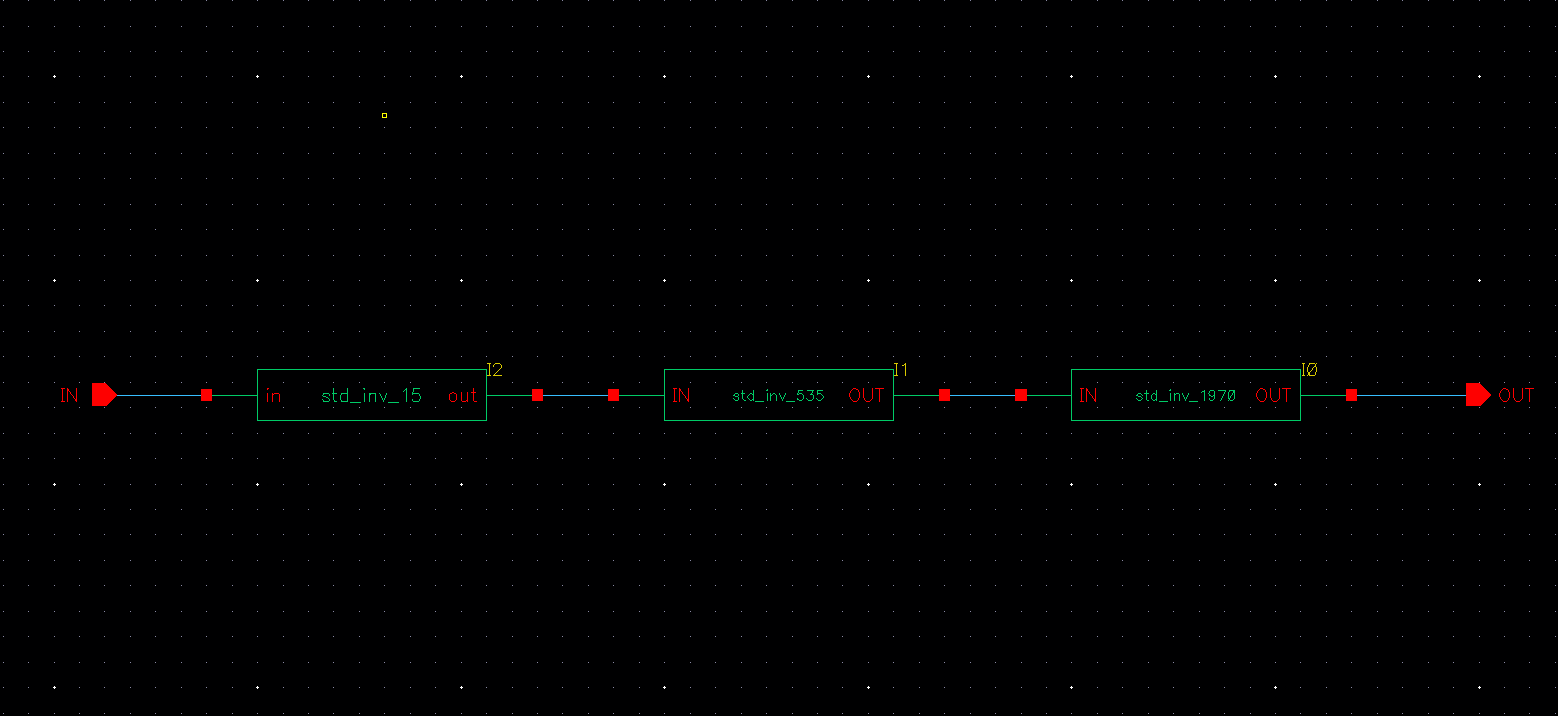
\includegraphics[width=1.0\linewidth]{inv_chain_3_schematic.png}
	\caption{Schematic of the Inverter Chain}
	\label{fig1}
\end{figure}

After the schematic is created, the entire chain is simulated in the ADE L tool (shown in Figure \ref{fig2} and \ref{fig3}).

% INSERT INVERTER CHAIN SCHEMATIC SIMULATION
\begin{figure}[htb!]
	\centering
	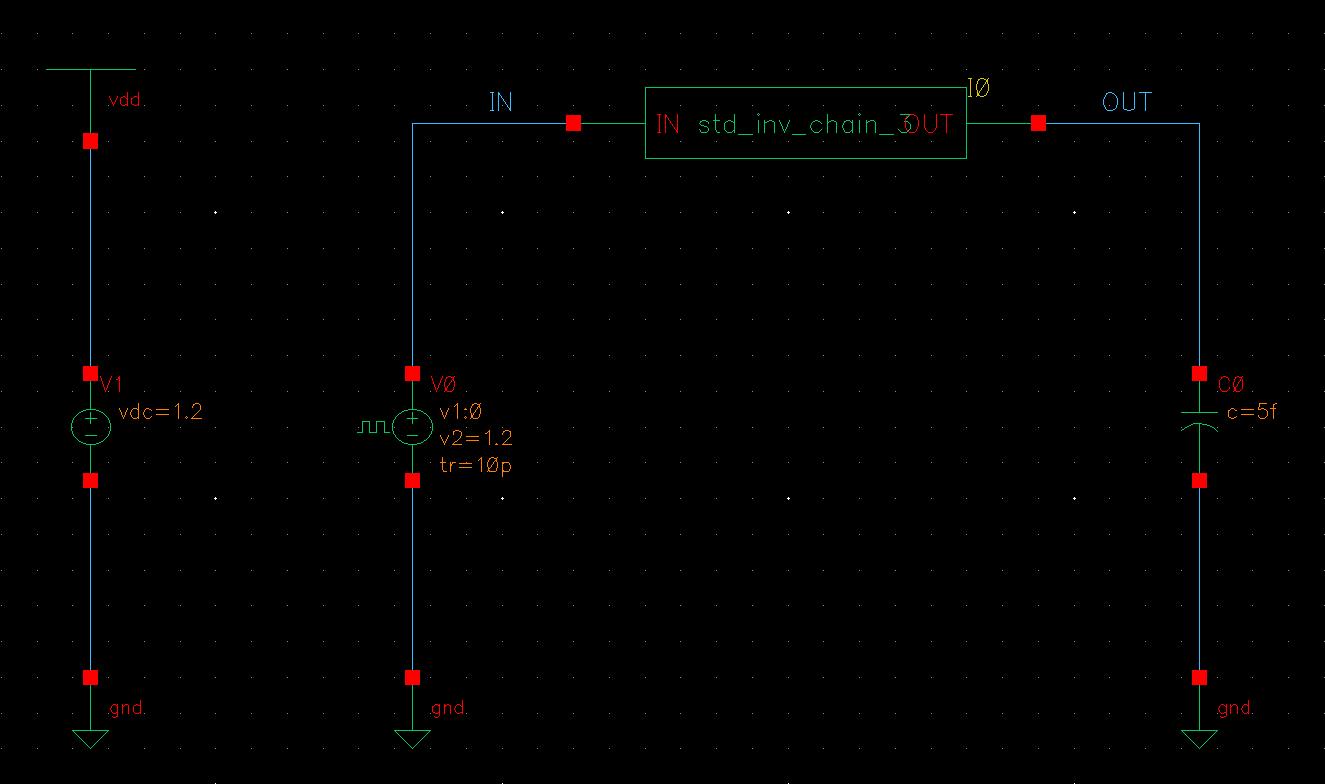
\includegraphics[width=1.0\linewidth]{inv_chain_3_schematic_sim.png}
	\caption{Schematic of the Inverter Chain's Transient Response Simulation}
	\label{fig2}
\end{figure}

\pagebreak
% INSERT INVERTER CHAIN ADE L SIMULATION RESULT (PRE-PEX)
\begin{figure}[htb!]
	\centering
	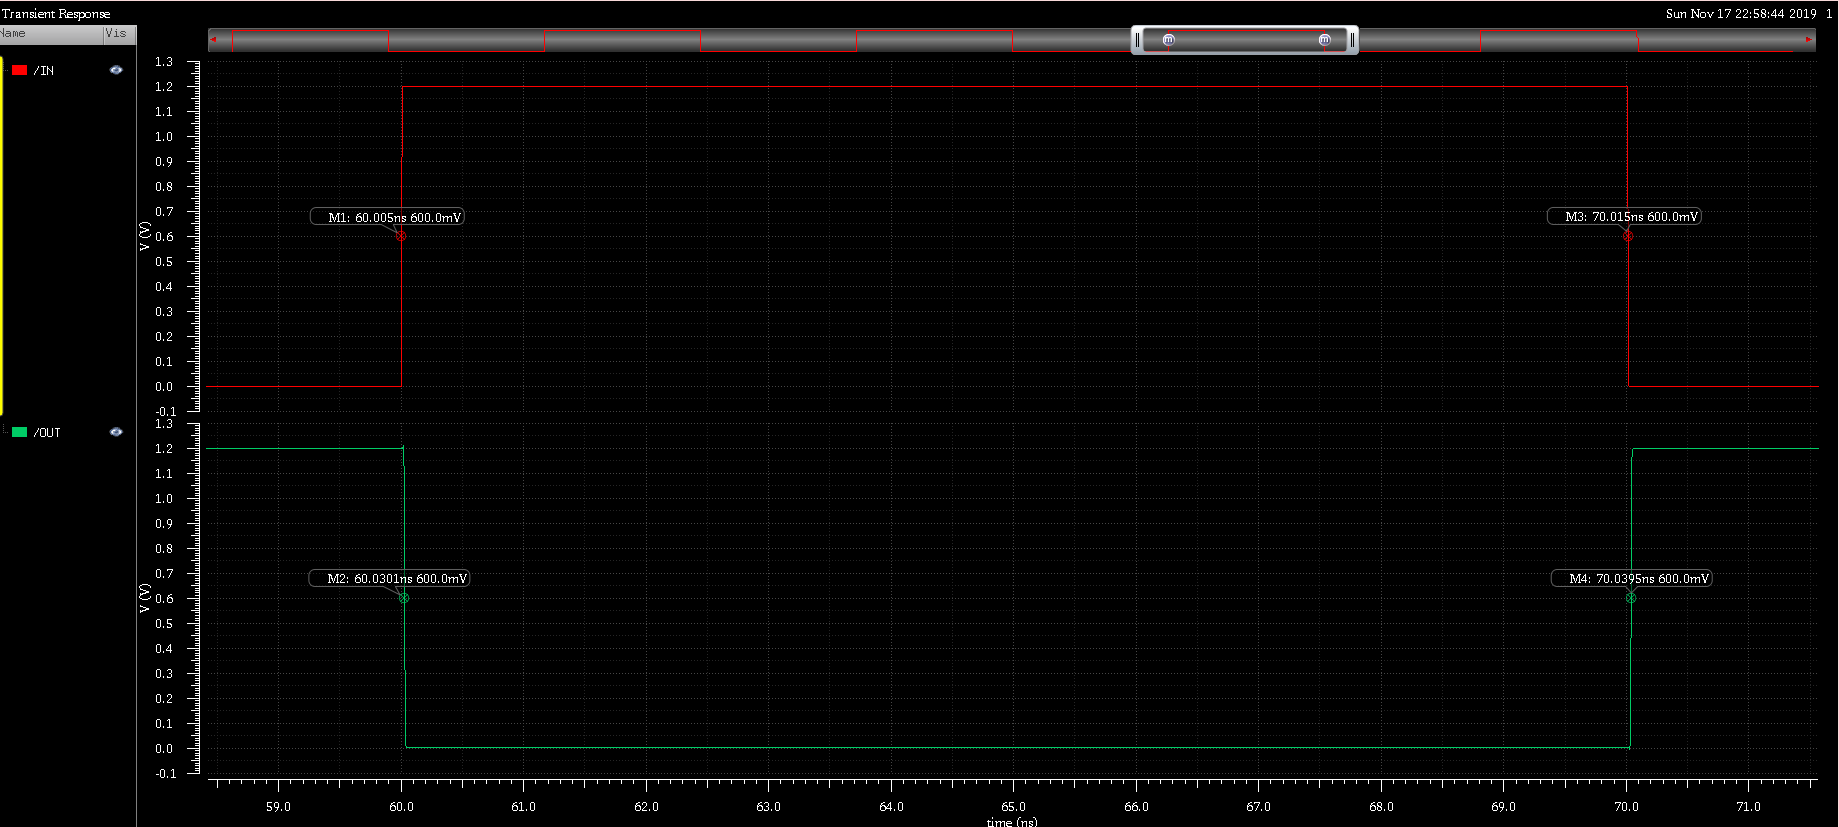
\includegraphics[width=1.0\linewidth]{inv_chain_3_prop_delay.png}
	\caption{The Inverter Chain's Transient Response Waveform with Markers indicating its propagation delay}
	\label{fig3}
\end{figure}

The propagation delay of the inverter chain is measured in Figure \ref{fig3}:

\begin{math}\label{eq6}
\begin{array}{l}
t_{pdr} = 70.0395 - 70.015 = 0.02450ns\\
t_{pdf} = 60.0301 - 60.005 = 0.02510ns\\
t_{pd} = 0.02480ns
\end{array}
\end{math}

The result above, however, does not take into account other factor affecting the delay, such as: intrinsic capacitance, long interconnects and real-parasitic contribution due to a particular layout design. Hence, the better approximation of the delay will come in the post-layout simulation, detailed in the Post-Layout Simulation and Results Section.

\section{Layout Design and Verification Results}
\label{sec:layout_desg_and_verification}

This section details the layout of the inverter chain. Similar to the schematic, the layout connects 3 inverters with increasing sizes (\textbf{145nm/90nm, 535nm/330nm, 1970nm/1220nm}). The final layout is shown in Figure \ref{fig4} below:

% INSERT INVERTER CHAIN LAYOUT
\begin{figure}[htb!]
	\centering
	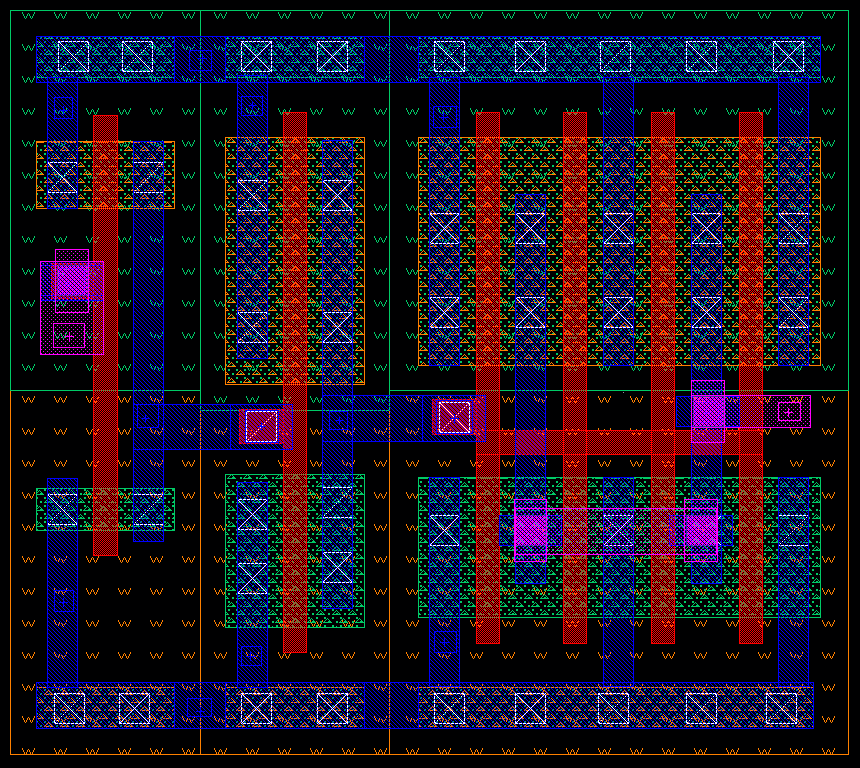
\includegraphics[width=0.7\linewidth]{inv_chain_3_layout.png}
	\caption{Layout of the Inverter Chain in Cadence's Virtuoso Layout Suite}
	\label{fig4}
\end{figure}

\pagebreak

The physical verifications of the layout above is shown in Figure \ref{fig5a} and \ref{fig5b}.

% INSERT DRC AND LVS
\begin{figure}[ht!]
	\centering
	\begin{subfigure}[b]{.48\linewidth}
		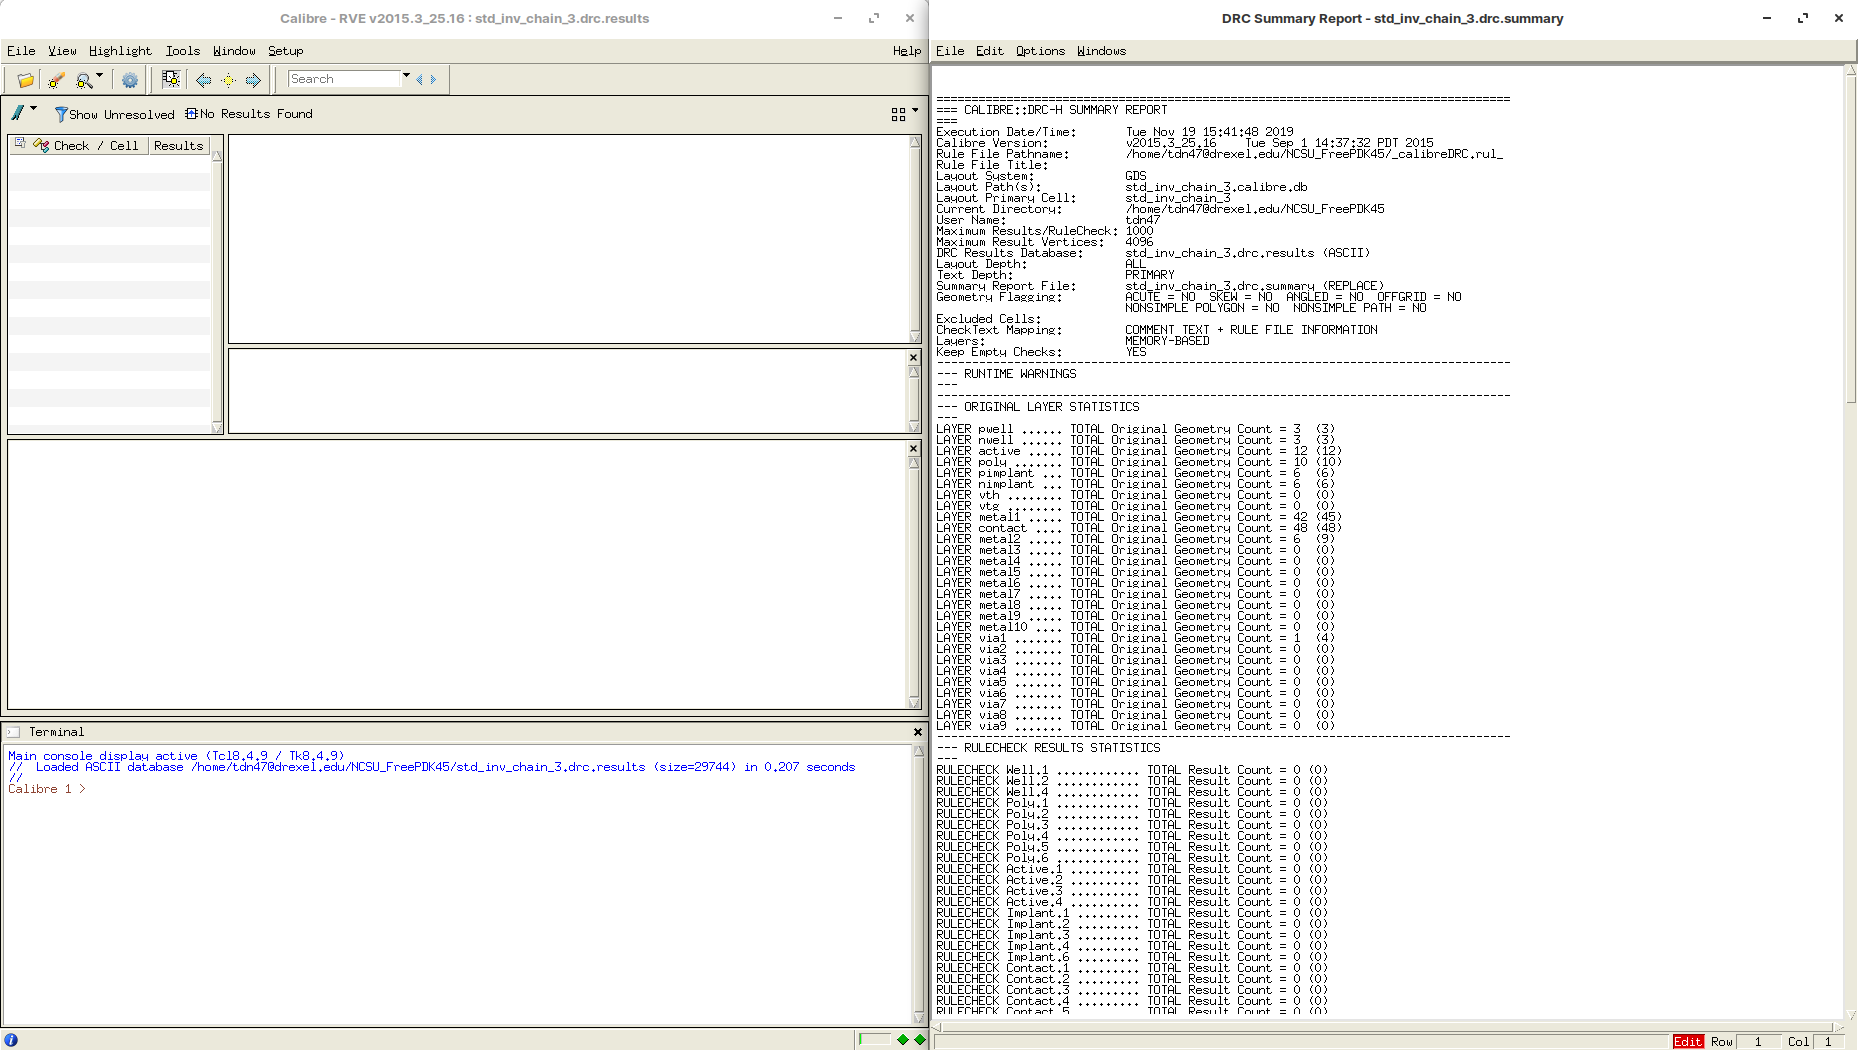
\includegraphics[width=\textwidth]{inv_chain_3_drc.png}
		\caption{DRC Verification Result}
		\label{fig5a}
	\end{subfigure}
%	\hskip2em
	\begin{subfigure}[b]{.48\linewidth}
		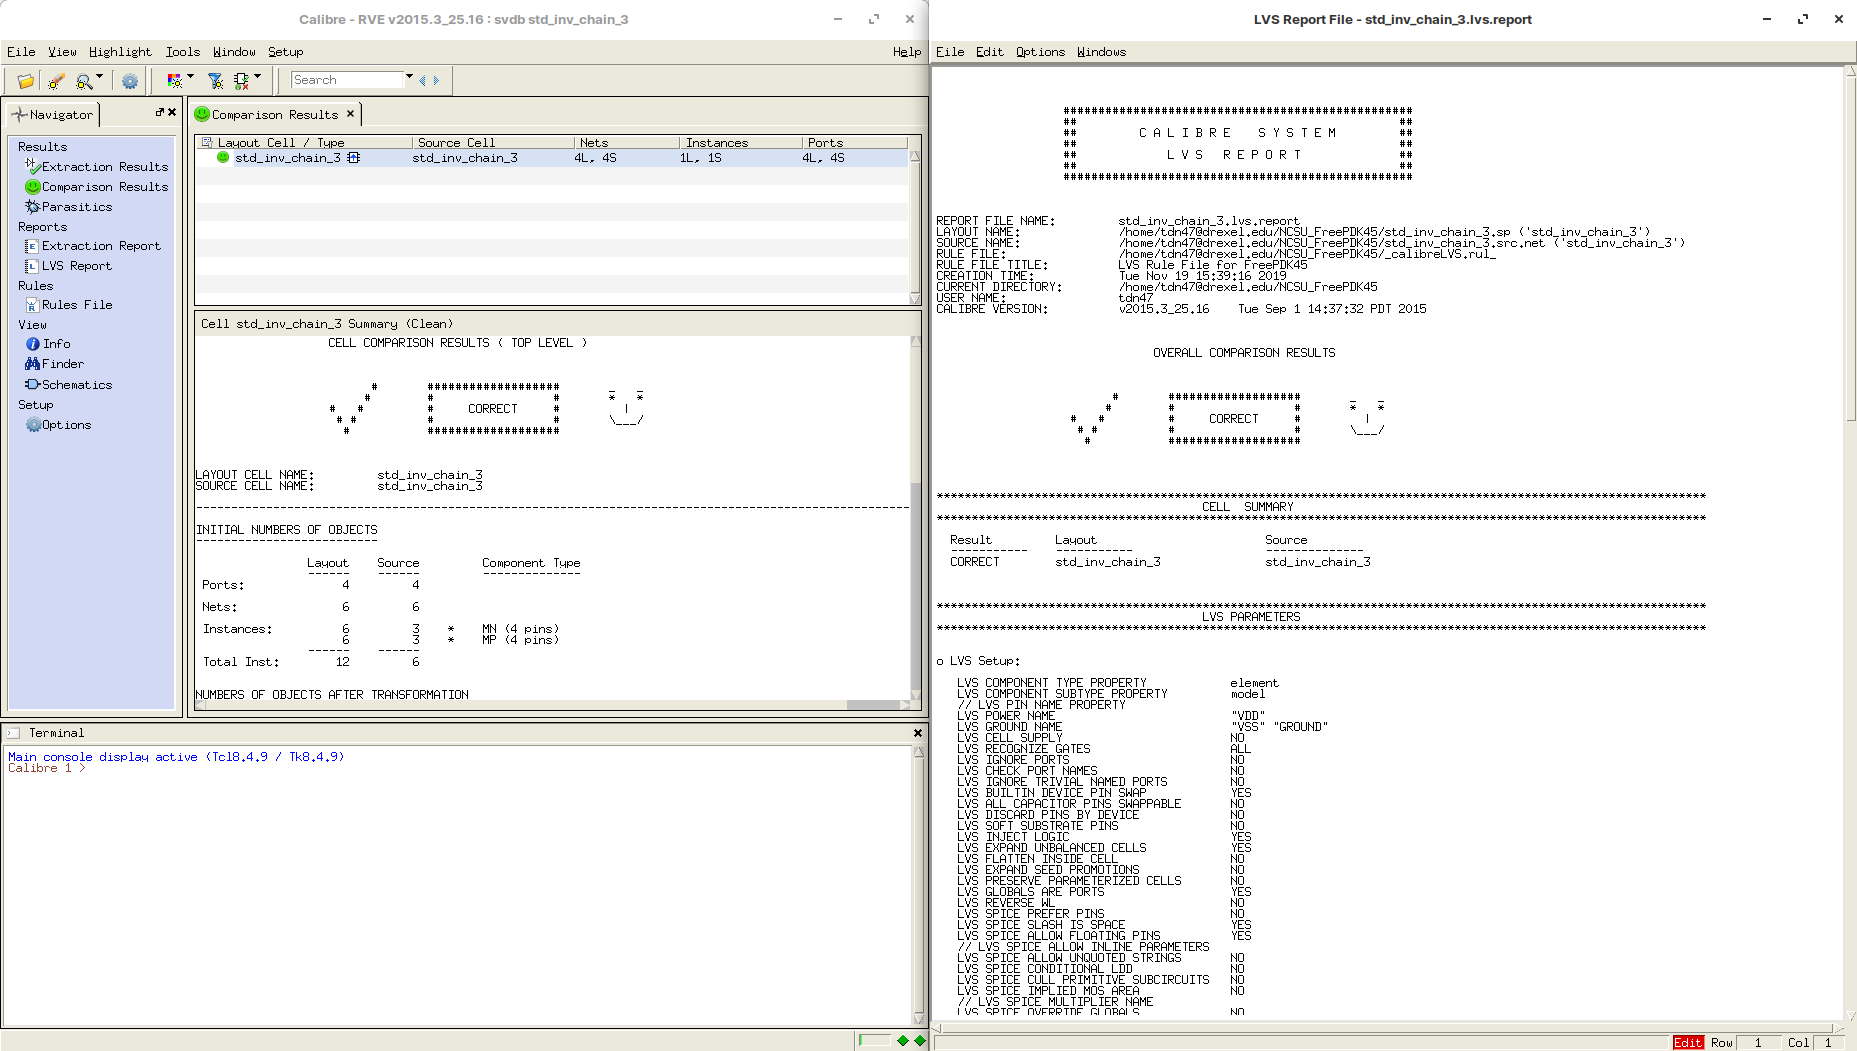
\includegraphics[width=\textwidth]{inv_chain_3_lvs.png}
		\caption{LVS Verification Result}
		\label{fig5b}
	\end{subfigure}
	\caption{Physical Verification Results using Cadence's Virtuoso Layout Suite}
\end{figure}

This layout will be used to generate the Post-Layout Simulation using Cadence Virtuoso Layout's PEX Calibre tool, which will account for all additional resistance and capacitance induced from this particular layout.


\section{Post-Layout Simulation and Results}
\label{sec:post_layout_simulation_results}

The PEX Calibre tool generates a Calibre View of the corresponding layout, which includes many parasitic resistors and parasitic capacitors (Figure \ref{fig6})

% INCLUDE PEX CALIBRE VIEW
\begin{figure}[htb!]
	\centering
	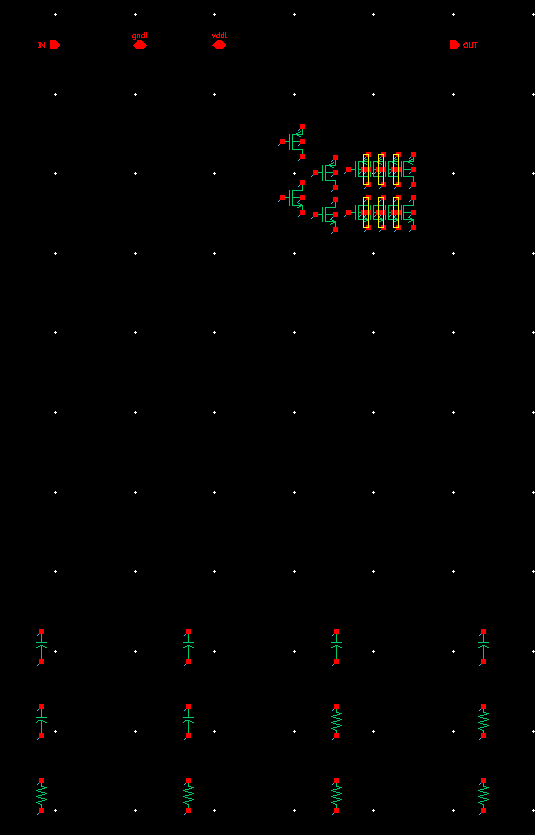
\includegraphics[width=0.35\linewidth]{inv_chain_3_calibre_view.png}
	\caption{Layout of the Inverter Chain After performing PEX Calibre View extraction}
	\label{fig6}
\end{figure}

With the extracted view, the ADE L simulation is re-ran and the propagation delay is re-evaluated (Figure \ref{fig7})

% INCLUDE INVERTER CHAIN TRANSIENT WITH CALIBRE
\begin{figure}[htb!]
	\centering
	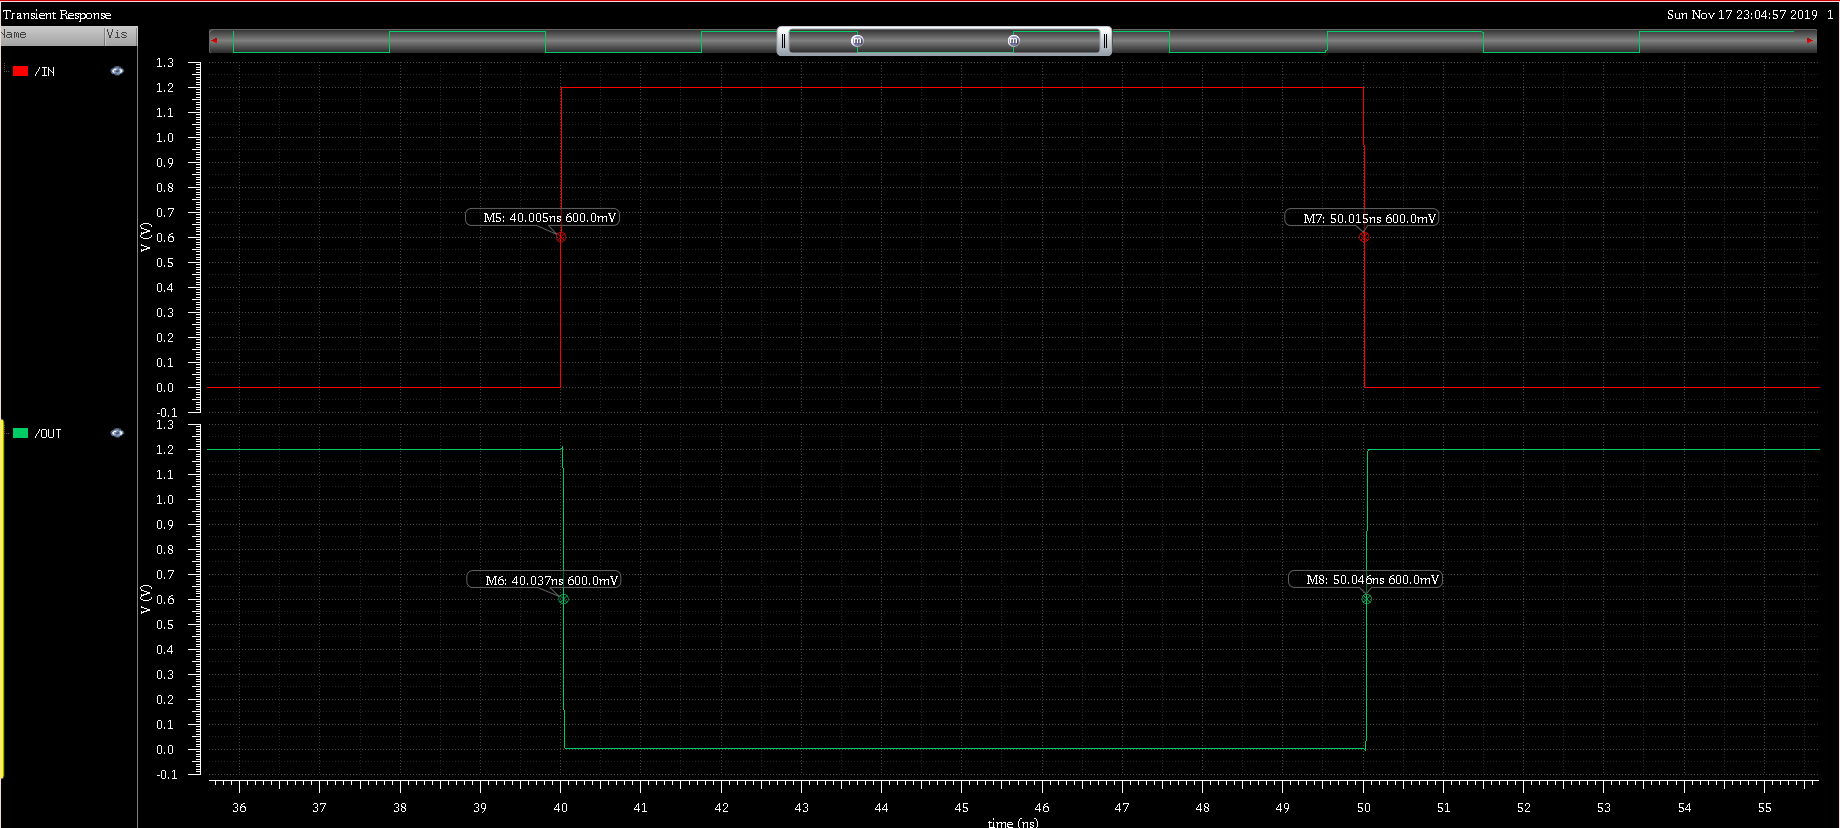
\includegraphics[width=0.85\linewidth]{inv_chain_3_calibre_prop_delay.png}
	\caption{Transient Response of the Inverter Chain After performing PEX Calibre View extraction}
	\label{fig7}
\end{figure}

\pagebreak

The propagation delay of the Post-Layout Simulation is:

\begin{math}\label{eq7}
\begin{array}{l}
t_{pdr} = 50.046 - 50.015 = 0.03100ns\\
t_{pdf} = 40.037 - 40.005 = 0.03200ns\\
t_{pd} = 0.03150ns
\end{array}
\end{math}

\section{Discussion and Conclusion}
\label{sec:disc_and_concl}

Considering the 2 propagation delay in Equation \ref{eq6} and \ref{eq7}, it is clear that the delay of the post-layout simulation is larger than that of the pre-layout one ($0.03150 > 0.02480$). Although in Equation \ref{eq3}, the parasitic contribution is assumed to be 0.5, this number is just an estimation. Hence, the fact that when parasitic capacitance and resistance due to connecting wires is accounted, the propagation delay increases, is obvious. 


\part{Ring Oscillator}
\label{part2}

\section{Schematic Simulation and Results}

The Ring Oscillator featured in this laboratory composed of 21 identically single-sized inverters. Connecting all of the inverters create the schematic shown in Figure \ref{fig8}.

% RING OSCILLATOR SCHEMATIC
\begin{figure}[htb!]
	\centering
	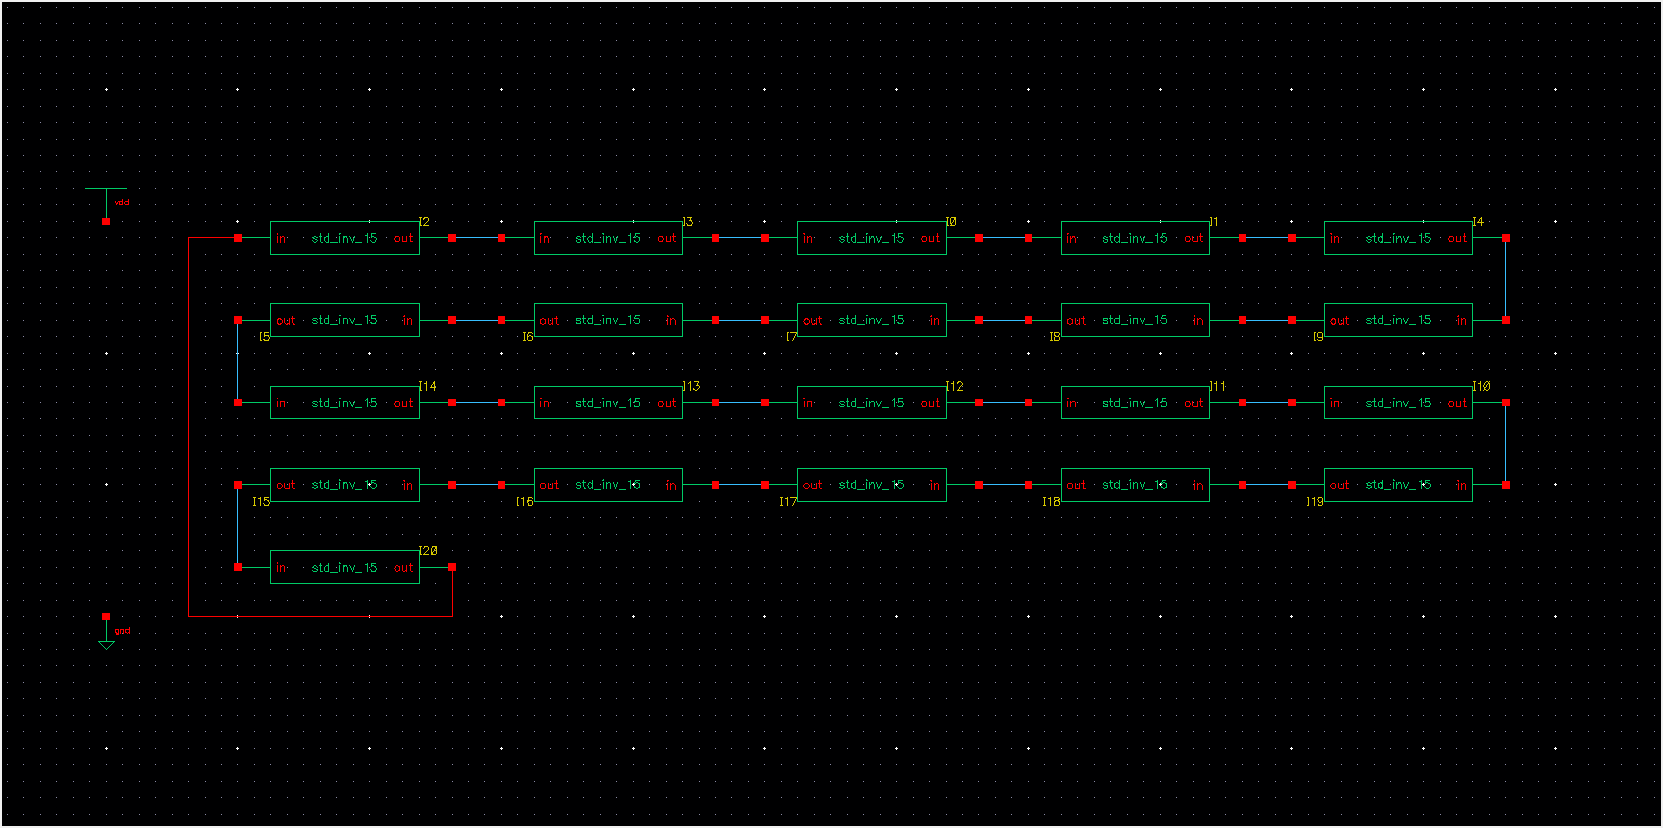
\includegraphics[width=0.7\linewidth]{ring_osc_schematic.png}
	\caption{Schematic of the Ring Oscillator}
	\label{fig8}
\end{figure}

The simulation for this schematic is done by injecting a stimulus to the system and recording the output's transient response (shown in Figure \ref{fig9}).

% RING OSCILLATOR TRANSIENT RESPONSE
\begin{figure}[htb!]
	\centering
	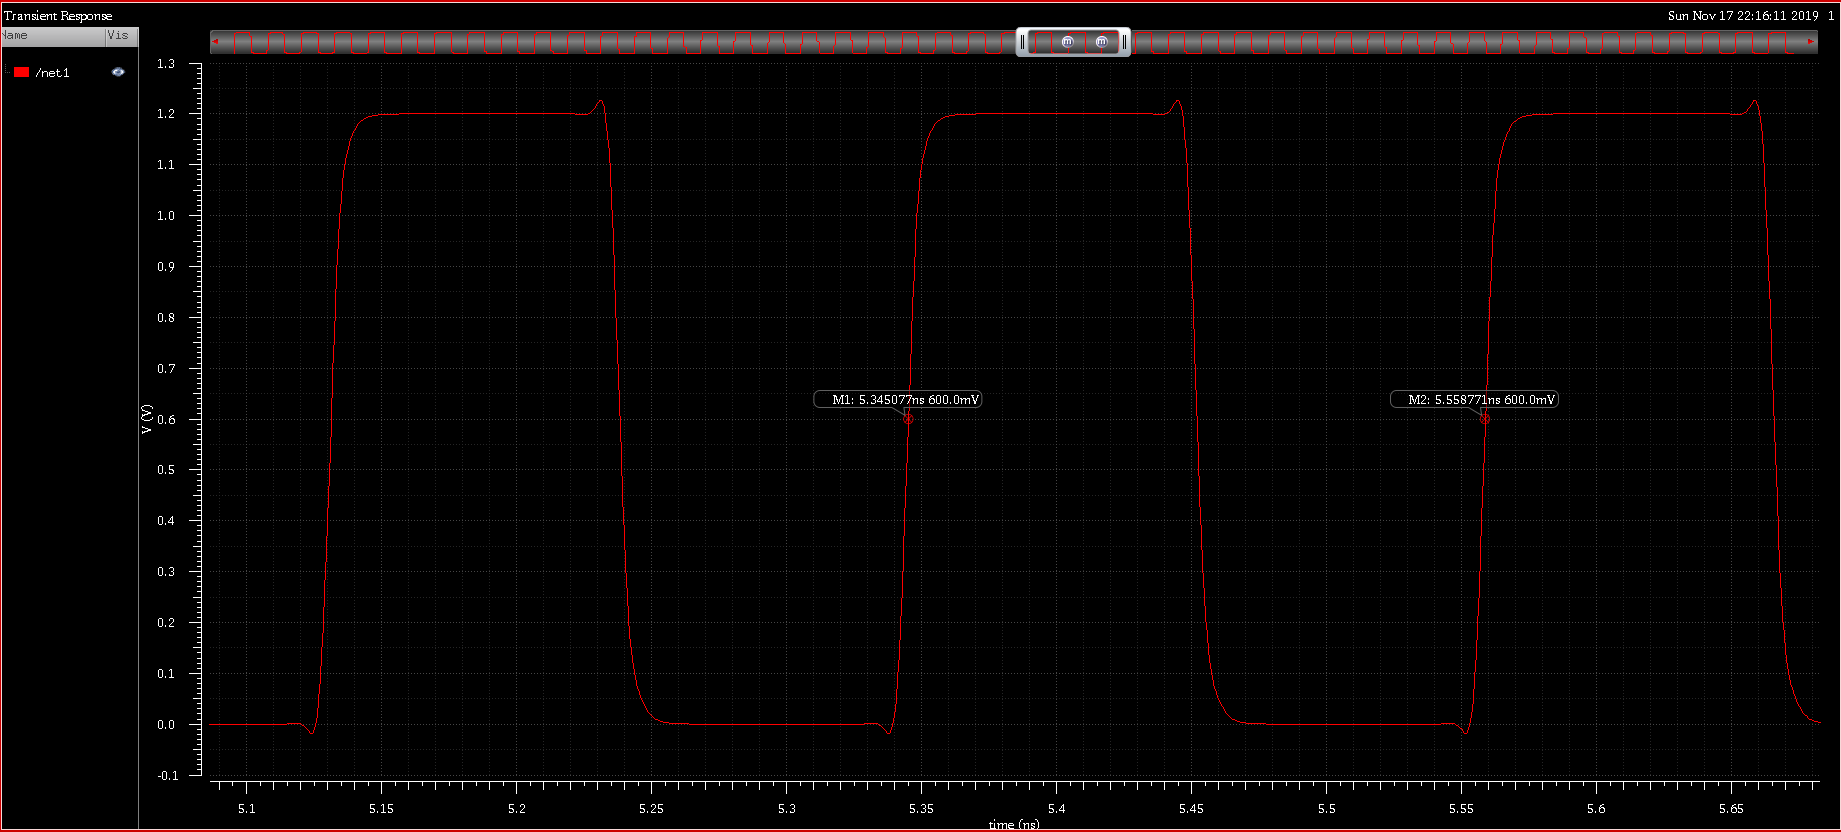
\includegraphics[width=0.75\linewidth]{ring_osc_clock_period.png}
	\caption{Transient Response of the Ring Oscillator with markers indicating clock period}
	\label{fig9}
\end{figure}

From the figure above, the clock's period can be measured:
\begin{equation}
period = 5.558771 - 5.5345077 = 0.21369ns
\end{equation}

And the frequency of the clock is:
\begin{equation}\label{eq8}
f_{osc} = \frac{1}{0.21369\times10^{-9}s} = 4.67967 GHz
\end{equation}

Knowing the approximation equation for the frequency of the oscillator:
\begin{equation}\label{eq9}
f_{osc} = \frac{1}{2\times N\times d} = \frac{1}{2\times 21 \times 2 \times \tau} = \frac{1}{42\times \tau}
\end{equation}

From Equation \ref{eq8} and \ref{eq9}, $\tau$ (the delay of 1 inverter) is: $5.08ps$.

And, the delay of 1 inverter measured from the simulation is $2.678997-2.673959 = 5.04ps$ (shown in Figure \ref{fig10})
\begin{figure}[htb!]
	\centering
	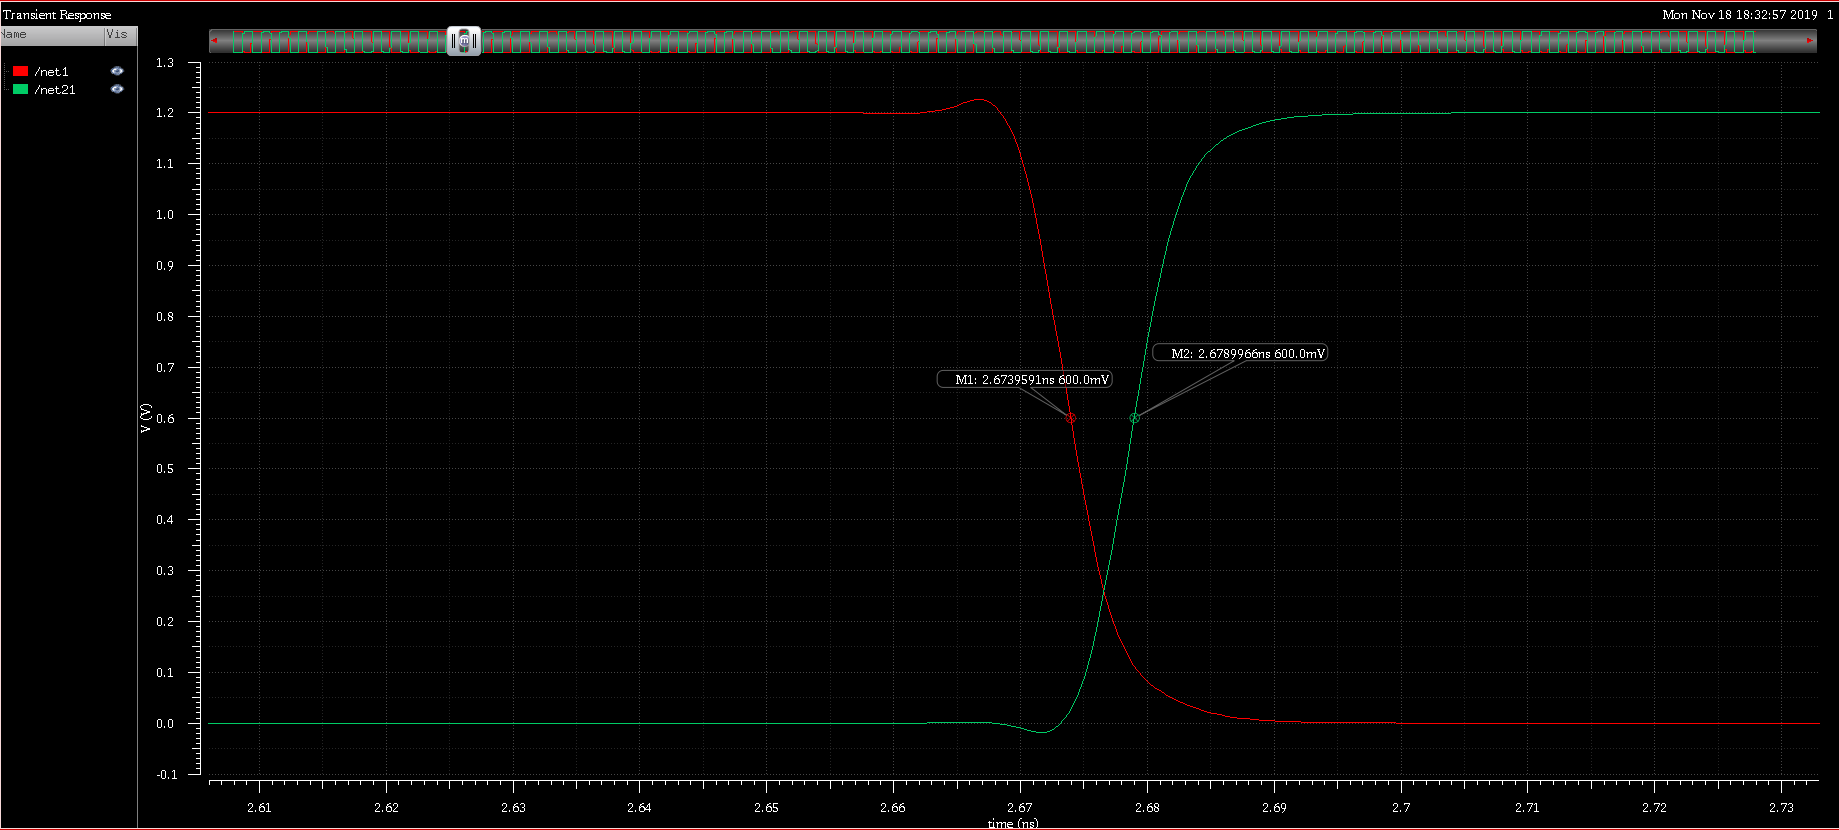
\includegraphics[width=0.75\linewidth]{ring_osc_inv_delay.png}
	\caption{Inverter delay of the Ring Oscillator with markers indicating the delay time}
	\label{fig10}
\end{figure}

\section{Discussion and Conclusion}

The results above show that the "theoretical" estimation is very close to the experimental measurements ($5.08ps$ and $5.04ps$). Hence, the ring oscillator behaves as expected.

\end{document}